\documentclass[fleqn, 10pt]{article}

% Paquetes necesarios
\usepackage[utf8]{inputenc}
\usepackage{babel}[spanish]
\usepackage{amsthm, amsmath}
\usepackage{nccmath} %Para centrar ecuaciones
\usepackage{graphicx}
\usepackage{enumitem}
\usepackage{mathtools}

% Personalizo mi alfabeto
\DeclareMathAlphabet{\pazocal}{OMS}{zplm}{m}{n}
\newcommand{\Lb}{\pazocal{L}}

% Definimos los entornos para definiciones, teoremas, etc...
\theoremstyle{plain}
\newtheorem{proposicion}{Proposición}

\theoremstyle{definition}
\newtheorem{definition}{Definición}[section]
\newtheorem{example}{Ejemplo}[section]

%Definimos el título
\title{Teoría de Autómatas y Lenguajes Formales\\[.4\baselineskip]Práctica 2: Autómatas}
\author{Omar Lukach Temsamani}
\date{\today}

%Comienzo del documento
\begin{document}

%Generamos el título
\maketitle

\section{Descripción del autómata}

Se nos pide un DFA que solamente acepte la cadena "a". Queda tal que así:

  \begin{ceqn}	%Para definir ecuación centrada en el texto
    \begin{align*} %Ecuación multilínea con alineamiento personalizado (split y align)
    &K: \{q0, q1, q2\}\\
    &\Sigma :\{a,b\}\\
    &s: q0\\
    &F: q1\\
    &\delta: \{(q0, a, q1), (q0, b, q2), (q1,a,q2),(q1,b,q2),(q2,a,q2),(q2,b,q2)\}
    \end{align*} 
  \end{ceqn} 
  
\section{JFLAP - Diseño del autómata}

Tras diseñar el autómata en JFLAP, queda el siguiente diagrama:

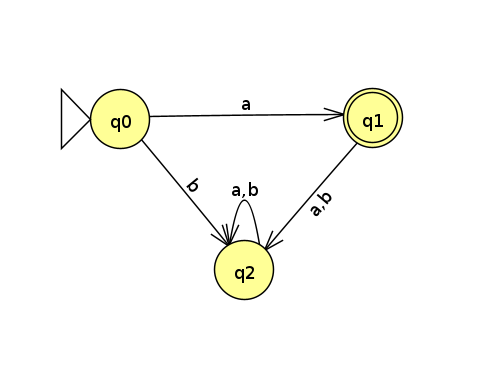
\includegraphics[height=212px]{/home/omar/RepoGit/PracticasTALF/Práctica 2/CapturaDFA.png}

\section{Octave - Testeo del autómata}

Tras modificar el archivo .json y probar el autómata en octave con una cadena apta ("a"), nos devuelve lo siguiente:\\
\\
\begin{ceqn}	%Para definir ecuación centrada en el texto
$M = (\{q_0, q_1, q_2\}, \{a, b\}, \{(q_0, a, q_1), (q_0, b, q_2), (q_1, a, q_2), (q_1, b, q_2), (q_2, a, q_2), (q_2, b, q_2)\}, q_0, \{q_1\})$

$w = a$

$(q_0, a) \vdash (q_1, \varepsilon)$

$x \in \Lb(M)\\
ans = 1
$\end{ceqn} 
\\
\\
Sin embargo, tras probar con otra cadena("aa", por ejemplo), pasa esto:
\\
\\
\begin{ceqn}	%Para definir ecuación centrada en el texto
$M = (\{q_0, q_1, q_2\}, \{a, b\}, \{(q_0, a, q_1), (q_0, b, q_2), (q_1, a, q_2), (q_1, b, q_2), (q_2, a, q_2), (q_2, b, q_2)\}, q_0, \{q_1\})$

$w = aa$

$(q_0, aa) \vdash (q_1, a) \vdash (q_2, \varepsilon)$

$x \notin \Lb(M)\\
ans = 0
$\end{ceqn} 
\\
\\
Vemos que para cadenas con más de una "a", el el script nos devuelve que la cadena no pertenece al lenguaje. al incluir una "b" pasará lo mismo:
\\
\\
\begin{ceqn}
$M = (\{q_0, q_1, q_2\}, \{a, b\}, \{(q_0, a, q_1), (q_0, b, q_2), (q_1, a, q_2), (q_1, b, q_2), (q_2, a, q_2), (q_2, b, q_2)\}, q_0, \{q_1\})$

$w = ab$

$(q_0, ab) \vdash (q_1, b) \vdash (q_2, \varepsilon)$

$x \notin \Lb(M) \\
ans = 0
$\end{ceqn} 
\\
\\ Y lo mismo si probamos con una cadena que empiece por "b":
\\

\begin{ceqn}
$M = (\{q_0, q_1, q_2\}, \{a, b\}, \{(q_0, a, q_1), (q_0, b, q_2), (q_1, a, q_2), (q_1, b, q_2), (q_2, a, q_2), (q_2, b, q_2)\}, q_0, \{q_1\})$

$w = ba$

$(q_0, ba) \vdash (q_2, a) \vdash (q_2, \varepsilon)$

$x \notin \Lb(M)$ \\
$ans = 0$
\end{ceqn} 



\end{document}